\documentclass[12pt,a4paper]{article}

\usepackage[utf8]{inputenc}
\usepackage[T1]{fontenc}
\usepackage{geometry}
\usepackage{setspace}
\usepackage{booktabs}
\usepackage{array}
\usepackage{amsmath}
\usepackage{hyperref}
\usepackage{natbib}
\usepackage{times}
\usepackage{microtype}
\usepackage{caption}
\usepackage{float}
\usepackage{graphicx}
\usepackage{tabularx}

\geometry{a4paper, margin=2.5cm}
\setstretch{1.5}
\hypersetup{colorlinks=true, linkcolor=blue, citecolor=blue, urlcolor=blue}

\title{\textbf{A Probabilistic Forecasting Benchmark\\for School Electricity Demand in South Africa}}
\author{}
\date{}

\begin{document}

\maketitle
\thispagestyle{empty}


\begin{abstract}
	Electricity represents a significant operational cost and source of financial risk for public schools in South Africa, particularly in lower-quintile communities where ageing infrastructure, load-shedding, and volatile network tariffs compound budgetary pressure and disrupt educational continuity. Whilst smart-meter deployments have enabled descriptive analytics and point-forecasting studies, there is still limited evidence on probabilistic forecasting for school electricity demand in resource-constrained settings. This paper establishes an operationally motivated probabilistic forecasting benchmark using a panel of 53 Western Cape schools with whole-building electricity consumption at 30-minute resolution \citep{samuels2025}. Multiple conditional quantiles are estimated using gradient-boosted quantile regression trained on the pinball loss, with calendar descriptors and seasonal autoregressive features as predictors. We compare independent per-school models with a pooled model that shares statistical strength across the panel via a categorical school-identifier feature, and also report a simple two-stage asymmetric width-calibration variant. Forecast quality is evaluated under 12-fold rolling-origin backtesting using median absolute error, mean pinball loss, empirical coverage at the 50\%, 80\%, and 90\% nominal levels, and 80\% interval width. A rolling-origin historical time-of-week quantile baseline is included as a transparent probabilistic reference. The results show a clear calibration--sharpness trade-off: the per-school model is more accurate and sharper, but under-covers; the pooled model achieves coverage closer to nominal, but with wider intervals and higher pinball loss; and the calibrated variant partially improves the pooled baseline without fully removing the trade-off. The resulting benchmark provides a reusable baseline for future hierarchical, weather-aware, load-shedding-aware, and decision-oriented extensions in an under-studied sub-Saharan African school setting.
\end{abstract}
\newpage


\section{Introduction}

Electricity expenditure has become central to the operational sustainability of public schools in South Africa, where rising network tariffs, recurring load-shedding, and heterogeneous infrastructure quality collectively threaten institutional budgets and educational continuity. In resource-constrained settings, even modest gains in demand predictability --- through improved scheduling of flexible loads, better-targeted retrofit investment, or more accurate utility budgeting --- can translate into material improvements in service continuity. \citet{samuels2025dataset} instrumented a cohort of Western Cape schools with smart meters and released a public dataset providing high-frequency whole-building electricity consumption alongside enriched contextual descriptors. Prior analyses have demonstrated the value of descriptive analytics, clustering, and benchmarking for characterising consumption patterns across heterogeneous school populations \citep{samuels2020, michaelahile2024}, but two unresolved methodological issues still limit the operational value of existing forecasting work.

The first issue concerns forecast output. As \citet{hongfan2016} argue, point forecasts are insufficient for planning tasks that require understanding the full distribution of future demand. \citet{haben2021} show empirically that studies reporting only point-forecast metrics provide an incomplete picture of model quality, and \citet{elhabyb2024} confirm that whilst machine learning outperforms statistical baselines for educational buildings, evaluation is restricted to RMSE and MAPE, leaving uncertainty uncharacterised. The second issue concerns cross-school structure. \citet{montero2021} establish that global (pooled) models enjoy substantially better generalisation bounds than local (per-school) models under finite-data conditions, and \citet{bentaieb2021} demonstrate that pooling across smart-meter hierarchies improves probabilistic forecast quality. Yet the building energy literature has not systematically examined whether probabilistic calibration is preserved under cross-site pooling in heterogeneous school settings, particularly in under-studied African contexts.

This paper addresses these two issues by applying quantile regression with gradient-boosted trees \citep{friedman2001, ke2017} to 30-minute demand data across 53 schools, using the pinball loss \citep{koenker1978} as the training objective and proper scoring rules \citep{gneitingraftery2007} for evaluation. Per-school models are compared with a pooled model augmented by a categorical school-identifier feature \citep{montero2021}, with all primary evaluation conducted under rolling-origin backtesting \citep{hyndman2021}. A rolling-origin historical time-of-week quantile baseline is included to provide a transparent probabilistic reference, and a simple two-stage asymmetric width-calibration variant is reported to assess whether pooled-model interval calibration can be improved after fitting. The central research question is whether cross-school pooling improves probabilistic forecast quality, calibration, and interval sharpness relative to per-school models for half-hourly school electricity demand.

\subsection*{Contributions}

This paper makes three principal contributions. First, it provides a probabilistic forecasting benchmark for school electricity demand at half-hourly resolution using gradient-boosted quantile regression in an under-studied sub-Saharan African school setting. Second, it delivers a focused cross-school comparison of per-school, pooled, and two-stage calibrated variants assessed under rolling-origin backtesting on pinball loss, MAE, calibration diagnostics, and interval sharpness at three coverage levels, aligned with the evaluation needs highlighted in the low-voltage forecasting literature \citep{haben2021}. Third, it provides reusable evaluation artefacts --- including rolling-origin fold summaries, reliability curves, per-school MAE summaries, and a historical-quantile baseline script --- to support future modelling work on the dataset.

\section{Literature Review}

Short-term electricity demand forecasting at the building level has received growing attention as smart-metering infrastructure has matured, yet performance varies strongly with data volume, aggregation level, and whether the objective is point or probabilistic \citep{haben2021}. Educational buildings are a particularly challenging sub-class: their consumption profiles are governed by term calendars, occupancy schedules, and catering or air-conditioning loads, generating strong daily and weekly periodicities superimposed on term-time versus holiday switching effects that simple autoregressive models fail to capture. \citet{elhabyb2024} confirm that gradient-boosting and deep learning outperform statistical approaches for educational buildings, attributing this to their ability to represent non-linear interactions between time-of-day, day-of-week, and occupancy features.

The case for probabilistic over deterministic forecasting is well established in principle but inconsistently implemented in practice. \citet{hongfan2016} argue that point forecasts --- which dominated utility practice for over a century --- are inadequate for modern planning tasks. Quantile regression-based methods have attracted particular attention because they make minimal distributional assumptions and can be combined with any flexible non-parametric learner \citep{koenker1978}. Gradient-boosted trees have emerged as effective vehicles for quantile regression on tabular energy data, given their native support for quantile objectives and ability to model non-linear feature interactions without manual transformation \citep{friedman2001, ke2017}. Despite this, many published studies either report point outputs only, or restrict probabilistic evaluation to a single coverage level --- a substantive weakness since a model can appear well-calibrated at the median whilst systematically mis-covering the tails.

Evaluating probabilistic forecasts requires proper scoring rules that simultaneously reward calibration and sharpness. \citet{gneitingraftery2007} show that the Continuous Ranked Probability Score (CRPS) and the interval score are strictly proper, incentivising forecasters to issue their true predictive distribution. \citet{gneitingbal2007} introduce the probability integral transform (PIT) as a calibration diagnostic and formalise the paradigm of maximising sharpness subject to calibration. The pinball loss --- which approximates the CRPS when evaluated on a fine quantile grid --- was adopted as the primary metric in GEFCom2014 \citep{hong2016gefcom} and is now the de facto standard for probabilistic load forecast evaluation. Reliability diagrams complement aggregate scores by visualising, for each nominal level, whether empirical coverage matches the nominal target. A common pitfall is conflating in-sample fit with out-of-sample reliability: residual-based intervals underestimate true predictive uncertainty on held-out data \citep{he2022}. Time series cross-validation must also use rolling-origin evaluation to respect temporal dependence \citep{hyndman2021}.

The multi-series forecasting problem --- how to exploit panel data from many buildings --- has received substantial theoretical attention. \citet{montero2021} show that global models are not intrinsically more restrictive than local models and enjoy better generalisation bounds because complexity does not grow with the number of series. Including a school identifier as a categorical feature enables partial pooling: a shared functional form is learnt whilst school-specific adjustments are accommodated. \citet{candanedo2022} demonstrate empirically that global models outperform local models in a residential setting, and \citet{bentaieb2021} provide a formal hierarchical treatment for UK smart-meter data, showing that coherent probabilistic forecasts can be obtained across meter hierarchies through forecast combination. Transfer learning offers a related approach, though \citet{qian2024} caution that indiscriminate pooling from dissimilar source domains risks negative transfer.

Despite this body of work, few published studies combine probabilistic whole-building forecasting with proper scoring rules, a principled per-school versus pooled comparison, and multi-level calibration diagnostics for a heterogeneous school panel in a non-OECD context. The present study contributes a benchmark in that setting.

\begin{table}[H]
\centering
\caption{Summary of key literature cited in this review.}
\label{tab:litreview}
\small
\begin{tabular}{p{4.8cm} p{2.4cm} p{3.2cm} p{2.4cm} p{1.6cm}}
\toprule
\textbf{Paper} & \textbf{Data} & \textbf{Method} & \textbf{Metric(s)} & \textbf{Calibration discussed?} \\
\midrule
Hong \& Fan (2016) \textit{IJF} 32(3) & System load & Tutorial review & Pinball, CRPS, PIT & Yes \\
Koenker \& Bassett (1978) \textit{Econometrica} & General & QR theory & Pinball loss & No \\
Gneiting \& Raftery (2007) \textit{JASA} & General & Proper scoring & CRPS, interval score & Yes \\
Gneiting et al.\ (2007) \textit{JRSS-B} & Weather & Calib.--sharpness & PIT, reliability & Yes \\
Haben et al.\ (2019) \textit{IJF} 35(4) & 100 UK LV feeders & SARIMA, GAM, kNN & Pinball, CRPS & Partial \\
Haben et al.\ (2021) \textit{Appl.\ Energy} & LV smart meters & Review & Pinball, reliability & Partial \\
Ben Taieb et al.\ (2021) \textit{JASA} & UK smart meters & Hierarchical QR & PIT, CRPS & Yes \\
Montero-Manso \& Hyndman (2021) \textit{IJF} & M-competition & Global vs.\ local & MASE, sMAPE & No \\
He et al.\ (2022) \textit{Appl.\ Energy} & Power system & Quantile combination & Pinball, coverage & Partial \\
Makridakis et al.\ (2022) \textit{IJF} & Retail (M5) & LightGBM ensemble & Scaled pinball & No \\
Elhabyb et al.\ (2024) \textit{IJER} & Educational bldgs & GBM, LSTM & RMSE, MAPE & No \\
Qian et al.\ (2024) \textit{Build.\ Simul.} & Office (multi-site) & Transfer learning & RMSE, MAE & No \\
\bottomrule
\end{tabular}
\end{table}


\section{Data and Problem Setting}

The dataset comprises whole-building smart-meter electricity consumption from 53 lower- to middle-income schools in the Western Cape Province, South Africa \citep{samuels2025dataset}. Consumption is recorded at half-hourly resolution and expressed as kWh per 30-minute interval, yielding a high-frequency panel consistent with the form used in recent smart-meter forecasting literature \citep{haben2021, bentaieb2021}. Enriched contextual variables cover hour-of-day, day-of-week, month, season, school-term indicators, school-day flags, and holiday type classifications, which collectively encode the structured occupancy regime governing school consumption \citep{elhabyb2024, haben2019}.

Let $y_{s,t}$ denote consumption (kWh per interval) for school $s$ at time $t$, and $\mathbf{x}_{s,t}$ the feature vector. The objective is to estimate conditional quantiles
\begin{equation}
  \hat{Q}_q\!\left(y_{s,t} \mid \mathbf{x}_{s,t}\right), \quad q \in \{0.05,\,0.10,\,0.25,\,0.50,\,0.75,\,0.90,\,0.95\},
\end{equation}
defining 50\% ($\mathrm{P}_{25}$--$\mathrm{P}_{75}$), 80\% ($\mathrm{P}_{10}$--$\mathrm{P}_{90}$), and 90\% ($\mathrm{P}_{05}$--$\mathrm{P}_{95}$) prediction intervals. This multi-level structure follows the evaluation framework of GEFCom2014 \citep{hong2016gefcom} and the calibration-first paradigm of \citet{gneitingbal2007}.

Inter-school heterogeneity is considerable: schools differ in floor area, infrastructure age, catering provision, and air-conditioning availability, all of which shape the daily load profile. This heterogeneity makes the panel an instructive testbed for evaluating whether cross-site pooling preserves probabilistic calibration, particularly where some schools have shorter or more irregular metering histories.


\section{Methods}

\subsection{Feature Engineering}

Two families of predictors are constructed. The first comprises calendar and contextual features --- hour-of-day, day-of-week, month, season, school-term membership, school-day flags, and holiday type --- which encode the systematic components of the demand schedule and are standard in short-term building load forecasting \citep{haben2019, hongfan2016}. The second family comprises seasonal autoregressive features tailored to 30-minute resolution: short lags at 1 and 2 steps (30--60 min), a daily lag at 48 steps (24 h), and a weekly lag at 336 steps (7 days), together with rolling-mean features over daily and weekly windows. The same-hour-yesterday and same-hour-last-week lags directly address the two dominant periodicities of school consumption \citep{haben2019, bentaieb2021}. Weather and load-shedding covariates are not included in this initial benchmark because the aim is to isolate the pooling comparison within a feature set derived directly from the released school panel, rather than to combine pooling changes with external data integration. The results should therefore be interpreted as a calendar-and-autoregressive probabilistic baseline, not as a fully specified operational forecasting system. A warm-up region is excluded to ensure all lagged features are fully populated before the first training observation.

\subsection{Probabilistic Model}

For each quantile level $q$, a gradient-boosted quantile regressor minimises the pinball loss:
\begin{equation}
  L_q(y,\hat{y}) =
  \begin{cases}
    q\,(y - \hat{y}) & \text{if } y \geq \hat{y}, \\
    (1-q)\,(\hat{y} - y) & \text{if } y < \hat{y}.
  \end{cases}
\end{equation}
The pinball loss is a strictly proper scoring rule for quantile functionals \citep{koenker1978, gneitingraftery2007}, ensuring the optimal forecast is the true conditional quantile. Gradient-boosted trees are adopted for their strong performance on tabular energy data and native support for quantile objectives \citep{friedman2001, ke2017}. Prediction intervals at 50\%, 80\%, and 90\% are constructed from the corresponding quantile pairs.

\subsection{Per-School Versus Pooled Models}

Per-school models fit separate quantile regressors to each school's history, maximising school-specific fit but limited by individual data volumes. The pooled model is trained jointly on all 53 schools, exploiting cross-site regularisation to improve generalisation --- particularly for data-sparse schools. Following \citet{montero2021}, the complexity of a global model does not grow with the number of series, yielding tighter generalisation bounds. To accommodate inter-school heterogeneity within the pooled model, school identity is included as a categorical feature, enabling school-specific adjustments within a shared functional form --- a form of soft pooling \citep{bentaieb2021, makridakis2022}. In practical terms, this allows the boosted trees to split on school membership when that improves prediction, so common demand structure can be learnt across the full panel whilst still permitting school-specific offsets and interactions to emerge through the tree partitions. Both configurations use identical feature sets and quantile objectives, so performance differences are attributable to the pooling strategy.

As a secondary calibration layer, we also report a two-stage asymmetric width-calibration variant. This variant starts from the pooled quantile forecasts and rescales the distance between the median and the lower or upper interval bounds using calibration-fold coverage errors. For a lower--upper quantile pair $(q_L,q_U)$, the adjusted interval is
\begin{align}
\hat{Q}^{\mathrm{cal}}_{q_L} &= \hat{Q}_{0.50} - \lambda_L\left(\hat{Q}_{0.50}-\hat{Q}_{q_L}\right),\\
\hat{Q}^{\mathrm{cal}}_{q_U} &= \hat{Q}_{0.50} + \lambda_U\left(\hat{Q}_{q_U}-\hat{Q}_{0.50}\right),
\end{align}
where $\lambda_L$ and $\lambda_U$ are selected on calibration folds only and then applied to the held-out fold. The implementation uses asymmetric lower and upper scaling factors for the 80\% interval and applies the same calibrated scaling to the other reported intervals for evaluation. This variant is included as a diagnostic adjustment, not as a separate forecasting architecture.

\subsection{Evaluation Protocol}

Models are evaluated using 12-fold rolling-origin backtesting to preserve temporal ordering and reduce sensitivity to any single holdout period. In each fold, models are trained only on observations prior to the forecast origin and evaluated on the subsequent test window. We report mean $\pm$ standard deviation across folds for MAE at $\hat{Q}_{0.50}$ and seasonal naive baselines, together with mean pinball loss across all seven quantile levels, empirical coverage at 50\%, 80\%, and 90\% nominal levels, and mean 80\% interval width. The historical time-of-week quantile baseline is evaluated under the same rolling-origin protocol by estimating empirical quantiles from the training portion for each school, day-of-week, and half-hour slot. Following \citet{gneitingbal2007}, calibration and sharpness are treated as complementary: the preferred model maximises sharpness subject to calibration. Nominal-versus-empirical coverage curves provide a graphical calibration diagnostic across all three levels \citep{haben2021}, while Table~\ref{tab:results} reports the corresponding empirical coverage values directly.


\section{Results}

\subsection{Summary Metrics}

Table~\ref{tab:results} summarises the rolling-origin backtest results over 12 folds. The historical time-of-week quantile baseline provides a simple probabilistic reference, while the seasonal naive rows provide point-forecast references. The per-school quantile gradient-boosted model achieves the lowest MAE and mean pinball loss among the learning models, with MAE(P50) $1.006\pm0.330$ and mean pinball loss $0.299$. However, it under-covers at all three nominal levels, with empirical coverage of 0.437, 0.706, and 0.810 for the 50\%, 80\%, and 90\% intervals respectively. The pooled model improves empirical coverage, reaching 0.505, 0.796, and 0.895, but this comes with higher MAE, higher pinball loss, and wider 80\% intervals. The two-stage calibrated variant improves substantially over the pooled baseline in MAE, pinball loss, and interval width, while retaining 80\% coverage close to the pooled model. It therefore reduces part of the cost of pooling but does not dominate the per-school model on pinball loss or sharpness.

\begin{table}[H]
\centering
\caption{Rolling-origin backtest results over 12 folds. Seasonal naive baselines are point forecasts and therefore do not define probabilistic intervals. Historical quantiles are evaluated under the same rolling-origin protocol as the learning models.}
\label{tab:results}
\small
\begin{tabularx}{\textwidth}{>{\raggedright\arraybackslash}Xcccccc}
\toprule
\textbf{Method} & \textbf{MAE (P50)} & \textbf{Pinball} & \textbf{Cov.\ 50\%} & \textbf{Cov.\ 80\%} & \textbf{Cov.\ 90\%} & \textbf{Width 80\%} \\
\midrule
Seasonal naive (day, $y_{t-48}$)    & $1.163\pm0.380$ & N/A & N/A & N/A & N/A & N/A \\
Seasonal naive (week, $y_{t-336}$)  & $1.135\pm0.263$ & N/A & N/A & N/A & N/A & N/A \\
Historical quantiles (time-of-week) & $1.301\pm0.404$ & 0.380 & 0.439 & 0.708 & 0.805 & 3.368 \\
Per-school quantile GB              & $1.006\pm0.330$ & 0.299 & 0.437 & 0.706 & 0.810 & 2.747 \\
Pooled quantile GB                  & $1.441\pm0.517$ & 0.447 & 0.505 & 0.796 & 0.895 & 4.315 \\
Two-stage calibrated pooled GB      & $1.114\pm0.302$ & 0.369 & 0.542 & 0.790 & 0.864 & 3.806 \\
\bottomrule
\end{tabularx}
\end{table}

\subsection{Baselines and Fold-wise Differences}

The rolling-origin historical-quantile baseline strengthens the interpretation of the benchmark. It is fully probabilistic and uses only recurring time structure, yet it is outperformed by the per-school quantile GB model on MAE and pinball loss. This indicates that the gradient-boosted model captures useful non-linear structure beyond simple school-specific time-of-week quantiles. However, the historical baseline and the per-school model have similar coverage, confirming that under-coverage is not unique to the machine-learning model and may partly reflect school-level volatility in the rolling-origin evaluation windows.

To assess whether pooled learning differs meaningfully from per-school modelling under temporal variation, we compute paired fold-wise differences under rolling-origin backtesting and construct nonparametric bootstrap confidence intervals over folds. For MAE at the median (P50), the mean difference (pooled minus per-school) is 0.434 with a 95\% bootstrap confidence interval $[0.322,\,0.550]$. For mean pinball loss, the mean difference is 0.148 with a 95\% confidence interval $[0.104,\,0.193]$. For 80\% coverage, the mean difference (pooled minus per-school) is 0.090 with a 95\% confidence interval $[0.067,\,0.113]$. These intervals provide evidence that the observed trade-off is consistent across the evaluated rolling-origin folds: the pooled model is worse on MAE and pinball loss but better on empirical coverage. As a secondary comparison, the two-stage calibrated model improves upon the pooled baseline, with lower MAE, lower pinball loss, and narrower 80\% intervals, although it remains less sharp than the per-school model.

\subsection{Calibration and Reliability}

The reliability curves (Figure~\ref{fig:reliability}) should be read alongside the empirical coverage values in Table~\ref{tab:results}. The pooled model is close to nominal at all three reported levels, with empirical coverage of 50.5\%, 79.6\%, and 89.5\% against the 50\%, 80\%, and 90\% targets. By contrast, the per-school model is sharper but under-covers, especially at the 80\% and 90\% levels. The two-stage calibrated model reduces pooled-model width and pinball loss, but its 90\% coverage falls to 86.4\%, indicating that post-hoc sharpening comes with some loss of upper-tail coverage. The main empirical result is therefore not that pooling uniformly improves forecast quality, but that it shifts the calibration--sharpness balance.

\begin{figure}[htbp]
	\centering
	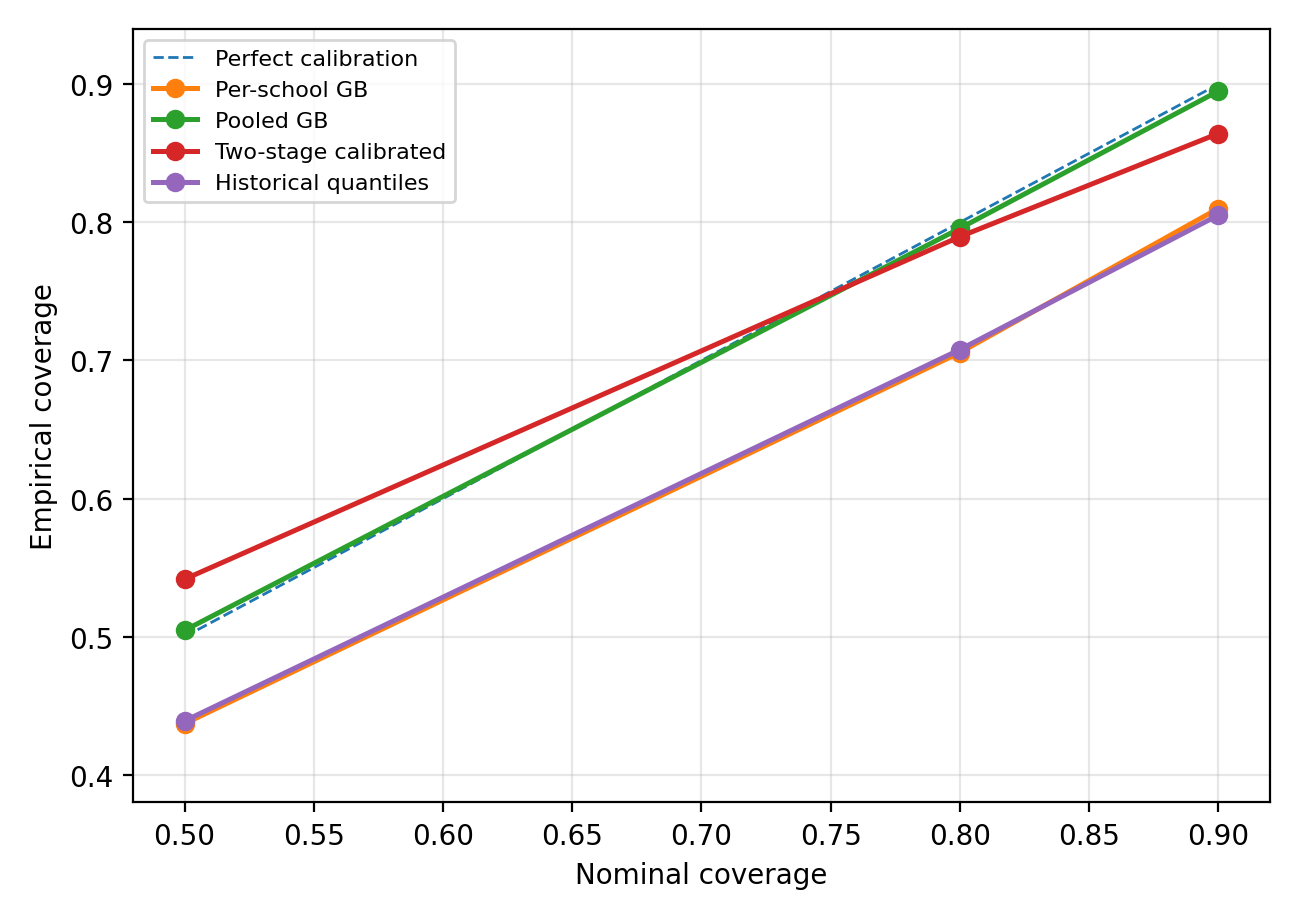
\includegraphics[width=0.9\textwidth]{wp1_conference_figure1_reliability.png}
	\caption{Reliability curves showing nominal versus empirical coverage for the rolling-origin historical-quantile baseline, per-school quantile GB, pooled quantile GB, and two-stage calibrated pooled model. The dashed diagonal indicates perfect calibration.}
	\label{fig:reliability}
\end{figure}

\subsection{Heterogeneity Across Schools}

Figure~\ref{fig:mae_by_school} shows the 20 schools with the highest average per-school MAE under rolling-origin evaluation, providing an illustrative ranking of harder-to-forecast buildings rather than a full distributional summary of all 53 schools. Figure~\ref{fig:mae_hist} complements this by showing the full distribution of per-school MAE values. The figures highlight that a subset of schools accounts for a disproportionate share of aggregate error, consistent with the heterogeneous profiles documented in the Western Cape dataset \citep{samuels2025dataset, michaelahile2024} and with multi-building forecasting literature showing that buildings with irregular occupancy or atypical consumption regimes are systematically harder to forecast \citep{haben2021}. These schools are precisely where better-calibrated uncertainty quantification and hierarchical extensions would provide the greatest benefit.

\begin{figure}[htbp]
	\centering
	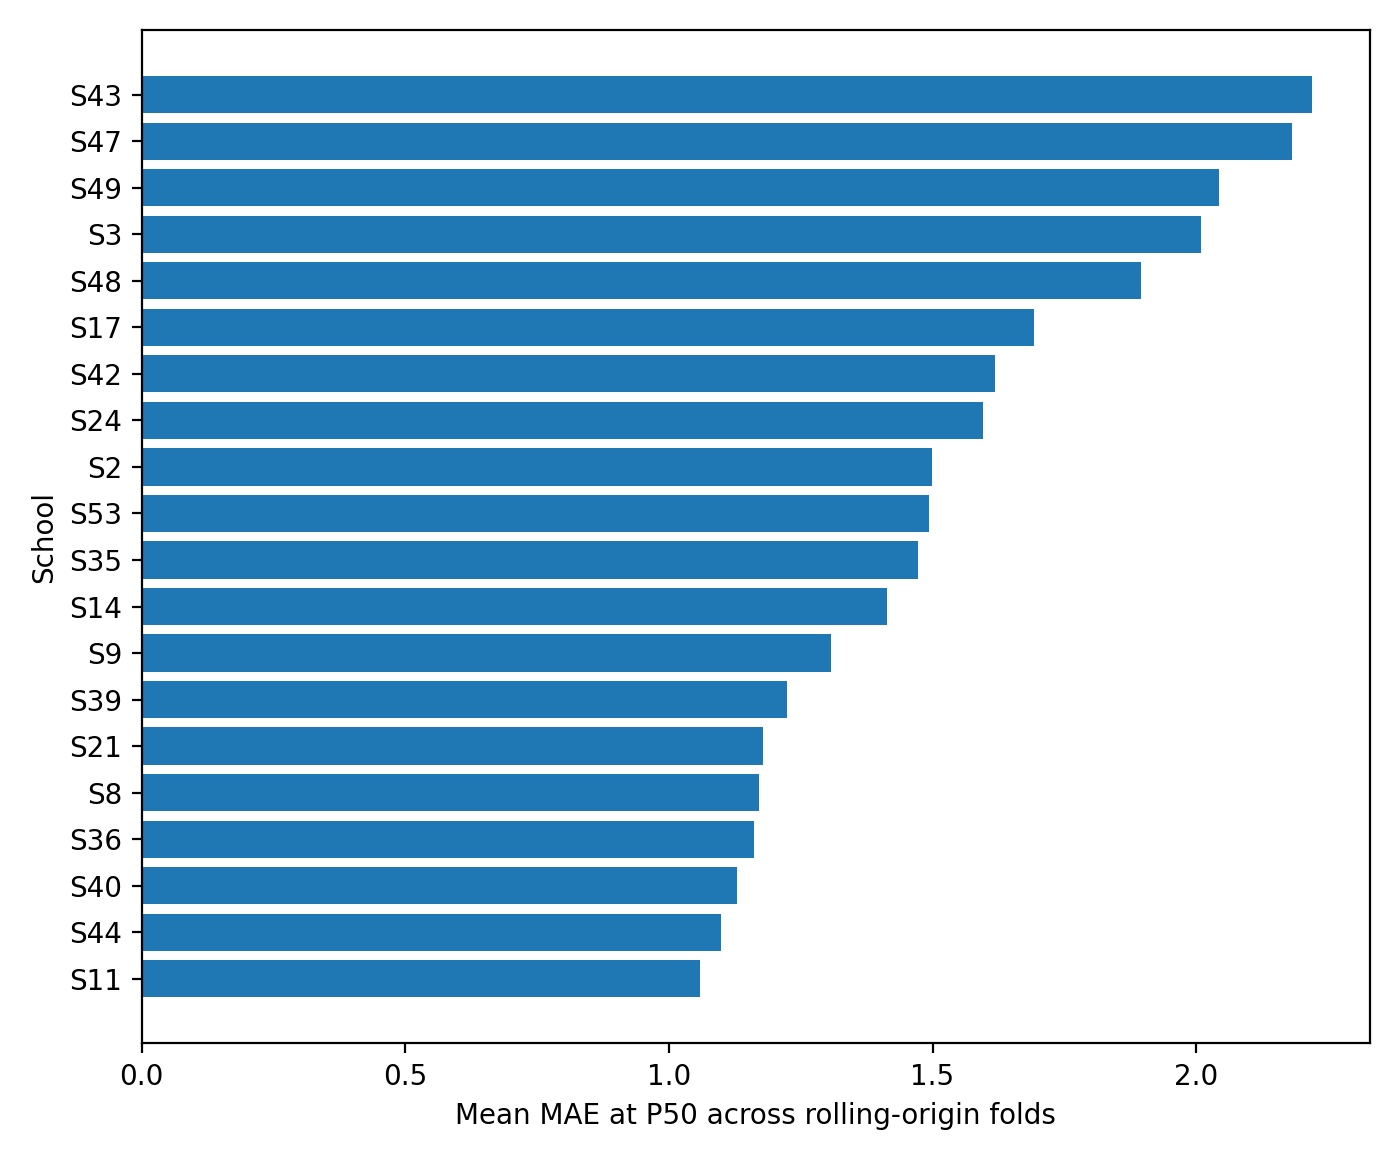
\includegraphics[width=0.8\textwidth]{wp1_conference_figure2_mae_top20.png}
	\caption{Top 20 schools with the highest mean per-school MAE at the predictive median across rolling-origin folds, illustrating heterogeneity in forecasting difficulty across the 53-school panel.}
	\label{fig:mae_by_school}
\end{figure}

\begin{figure}[htbp]
    \centering
    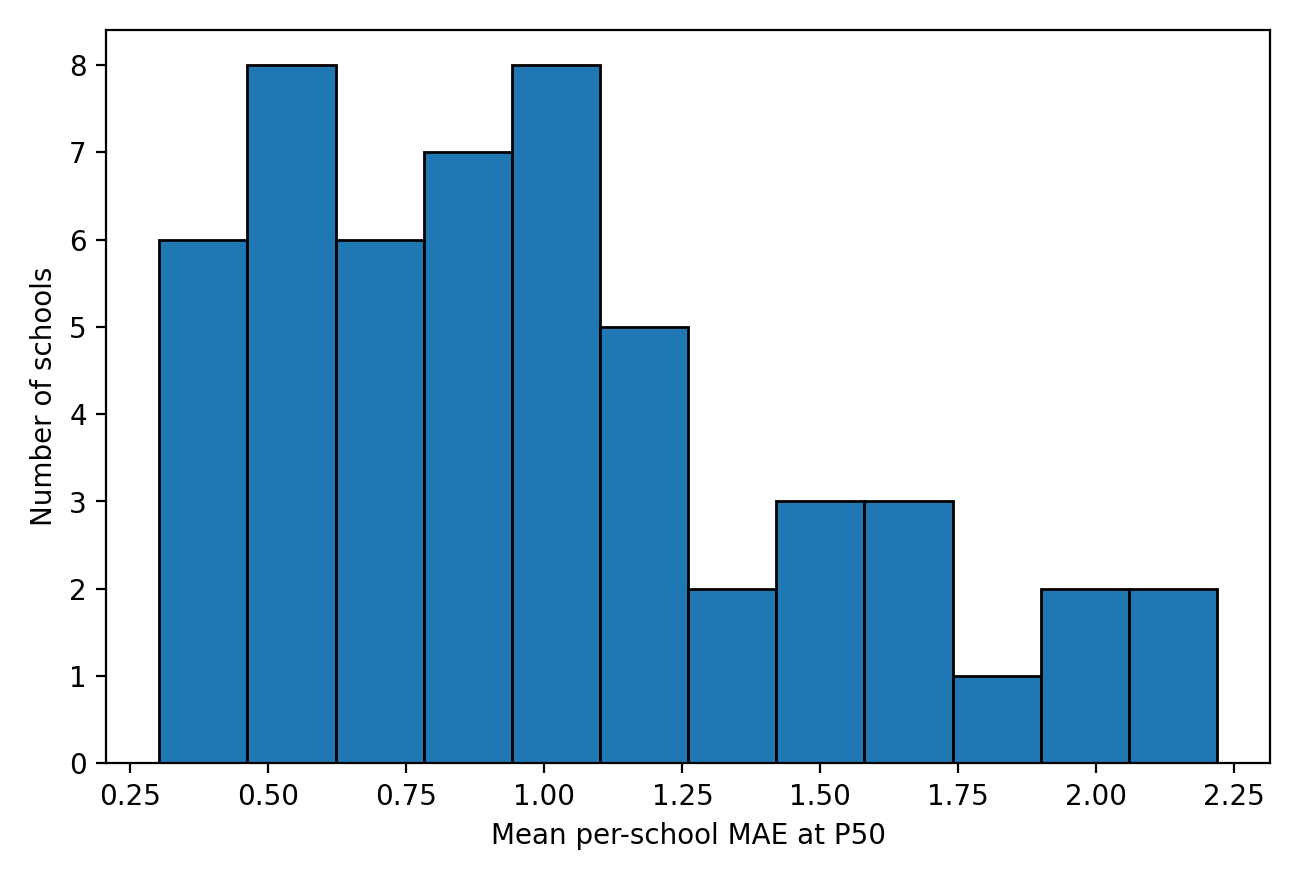
\includegraphics[width=0.75\linewidth]{wp1_conference_figure3_mae_distribution.png}
    \caption{Distribution of mean per-school MAE at the predictive median across the 53 schools.}
    \label{fig:mae_hist}
\end{figure}


\section{Discussion}

The results confirm that probabilistic forecasting of heterogeneous school electricity demand is achievable with computationally tractable models, provided features capture schedule-driven seasonality. They also show that cross-school pooling should not be interpreted as a simple improvement over local modelling. Instead, the rolling-origin evaluation reveals a calibration--sharpness trade-off. The per-school model achieves lower MAE, lower pinball loss, and narrower 80\% intervals, but it under-covers at the reported nominal levels. The pooled model achieves coverage closer to nominal, especially at the 80\% and 90\% levels, but this improvement is obtained through wider intervals and higher pinball loss. The two-stage calibrated variant partially improves the pooled baseline by reducing MAE, pinball loss, and interval width, but it does not fully remove the trade-off.

The inclusion of a rolling-origin historical-quantile baseline is important for interpreting the contribution. The per-school quantile GB model improves on this simple probabilistic baseline in both MAE and pinball loss, suggesting that the boosted model captures structure beyond recurring time-of-week effects. At the same time, the historical baseline provides a strong reminder that much of school electricity demand is schedule-driven. The contribution of this paper should therefore be understood as an operationally motivated benchmark and evaluation framework, rather than as a claim of algorithmic novelty.

This benchmark has four important limitations. First, the pooled model does not constitute a full hierarchical probabilistic model \citep{bentaieb2021}; a Bayesian hierarchical formulation would provide more principled uncertainty quantification for the harder-to-forecast schools in Figure~\ref{fig:mae_by_school} by modelling school-level effects as draws from a common prior. Second, although rolling-origin backtesting is used, the evaluation remains limited to 12 forecast origins and a fixed horizon specification; more extensive backtesting across alternative horizons and calendar regimes would strengthen the evidence on temporal robustness, particularly around term transitions \citep{hyndman2021}. Third, although load-shedding motivates the South African school context, explicit load-shedding stage variables are not included in this benchmark. Future work should incorporate planned and realised outage indicators to assess whether they improve tail calibration. Fourth, weather covariates were excluded in order to keep the initial benchmark focused on features available directly in the released school panel and to isolate the effect of pooling strategy, but their omission likely limits tail calibration during temperature extremes \citep{haben2019}. These extensions -- hierarchical modelling, broader rolling-origin evaluation, load-shedding integration, weather integration, and decision-focused use of probabilistic forecasts -- constitute a natural progression from the benchmark established here.

\section{Reproducibility and Artefacts}

All experiments are implemented in a self-contained pipeline that loads the enriched panel dataset \citep{samuels2025dataset}, constructs calendar and autoregressive features, trains quantile gradient-boosting models under the per-school, pooled, and two-stage calibrated configurations, and exports standardised reports and figures. The rolling-origin experiments produce \texttt{data/wp1\_rb\_overall\_summary.csv}, \texttt{data/wp1\_rb\_fold\_overall.csv}, and \texttt{data/wp1\_rb\_fold\_per\_school.csv}, which contain the fold-level and aggregate metrics reported in Table~\ref{tab:results}. The historical time-of-week quantile baseline is generated by a separate script and exported as \texttt{data/wp1\_rb\_historical\_quantile\_overall\_summary.csv} and \texttt{data/wp1\_rb\_historical\_quantile\_fold\_overall.csv}. Additional diagnostic artefacts include reliability curves and ranked MAE values for the hardest-to-forecast schools. The code, result CSVs, figures, and README are available in the project repository at \url{https://github.com/sanshumba/wp1}.

\section{Conclusion}

This paper presents a reproducible probabilistic forecasting benchmark for half-hourly whole-building electricity consumption across 53 lower- to middle-income schools in the Western Cape, South Africa. Gradient-boosted quantile regression with calendar and seasonal autoregressive features is evaluated under rolling-origin backtesting against seasonal naive and historical time-of-week quantile baselines. The results show that the per-school quantile GB model improves on the simple historical probabilistic baseline in MAE and pinball loss, but under-covers at the reported nominal levels. The pooled model achieves coverage closer to nominal but at the cost of wider intervals and worse MAE and pinball loss. A two-stage calibrated pooled variant improves on the pooled baseline but does not fully remove this calibration--sharpness trade-off.

For near-term use, the results suggest that per-school models may be preferable when point accuracy and sharper intervals are prioritised, while pooled or calibrated pooled variants may be more useful when aggregate coverage and risk screening are the main concern. Overall, the benchmark provides a practical baseline for future hierarchical, load-shedding-aware, weather-aware, and decision-oriented extensions in under-resourced school settings.


\bibliographystyle{apalike}
\IfFileExists{references_revised_final.bib}{\bibliography{references_revised_final}}{%
\begin{thebibliography}{}
\end{thebibliography}}

\end{document}
